\documentclass{beamer}
\usetheme{metropolis} 
\usepackage{graphicx}
\usepackage{tikz}
\usepackage{array}
\usepackage{booktabs}
\usepackage{subcaption} 
\usetikzlibrary{positioning, arrows.meta}
\usepackage{pgfplots}
\usepackage{xcolor}
\usepgfplotslibrary{groupplots}
\usetikzlibrary{patterns}
\usetikzlibrary{positioning, arrows.meta, shapes.geometric, shapes.misc}
\usetikzlibrary{positioning}
\usepackage{etex} % Extends TeX capacity
\maxdeadcycles=200 % Increase the limit of dead cycles
\usetikzlibrary{shapes, arrows.meta, decorations.pathreplacing, positioning}

\title{Neural Cleanse: Identifying and Mitigating Backdoor Attacks in Neural Networks}
\author{Niloy Das Robin}
\institute[CSE, BUET]{Department of CSE, BUET}
\date{\today}

\begin{document}

% \frame{\titlepage}

% Section 5
\section{Experimental Validation}
\subsection{Description of Datasets and Tasks Used for Evaluation}

% First Frame: Description of Datasets and Tasks
\begin{frame}{Description of Datasets and Tasks}
    \centering
    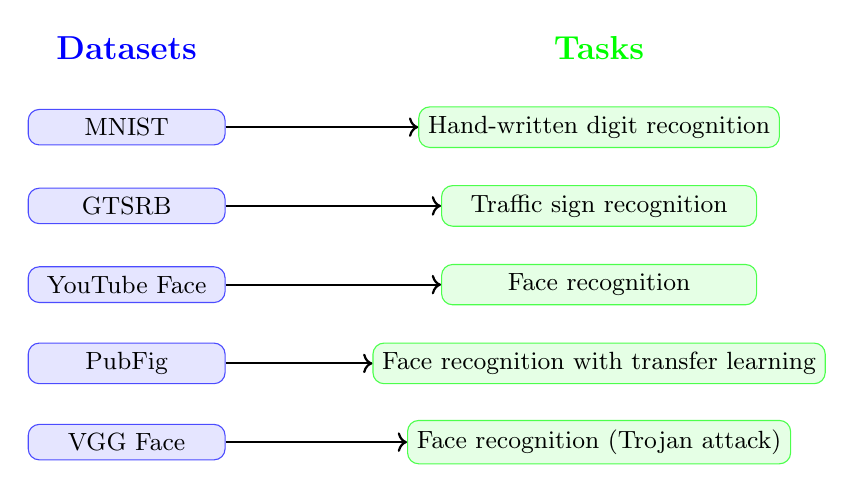
\begin{tikzpicture}[
        dataset/.style={rectangle, draw=blue!70, fill=blue!10, rounded corners, text centered, minimum width=2.5cm, font=\small},
        task/.style={rectangle, draw=green!70, fill=green!10, rounded corners, text centered, minimum width=4cm, font=\small},
        arrow/.style={->, thick}
    ]

        % Main Titles
        \node<1->[font=\large, text=blue] (datasets) at (0, 4) {\textbf{Datasets}};
        \node<1->[font=\large, text=green] (tasks) at (6, 4) {\textbf{Tasks}};

        % Datasets
        \node<1->[dataset] (mnist) at (0, 3) {MNIST};
        \node<2->[dataset] (gtsrb) at (0, 2) {GTSRB};
        \node<3->[dataset] (youtube) at (0, 1) {YouTube Face};
        \node<4->[dataset] (pubfig) at (0, 0) {PubFig};
        \node<5->[dataset] (vggface) at (0, -1) {VGG Face};

        % Tasks
        \node<1->[task] (digit) at (6, 3) {Hand-written digit recognition};
        \node<2->[task] (traffic) at (6, 2) {Traffic sign recognition};
        \node<3->[task] (face) at (6, 1) {Face recognition};
        \node<4->[task] (transfer) at (6, 0) {Face recognition with transfer learning};
        \node<5->[task] (trojan) at (6, -1) {Face recognition (Trojan attack)};

        % Arrows
        \draw<1->[arrow] (mnist.east) -- (digit.west);
        \draw<2->[arrow] (gtsrb.east) -- (traffic.west);
        \draw<3->[arrow] (youtube.east) -- (face.west);
        \draw<4->[arrow] (pubfig.east) -- (transfer.west);
        \draw<5->[arrow] (vggface.east) -- (trojan.west);

    \end{tikzpicture}
\end{frame}





% Second Frame: Table
\begin{frame}{Dataset and Model Details}
    \centering
    \scriptsize % Adjust font size to ensure table fits
    \begin{table} % Table environment
        \resizebox{\textwidth}{!}{ % Resize table to fit slide width
            \begin{tabular}{@{}>{\centering\arraybackslash}m{3.2cm}
                             >{\centering\arraybackslash}m{2.5cm}
                             >{\centering\arraybackslash}m{2.2cm}
                             >{\centering\arraybackslash}m{2.2cm}
                             >{\centering\arraybackslash}m{3.2cm}@{}}
                \toprule
                \textbf{Task} & \textbf{Dataset} & \textbf{\# of Labels} & \textbf{Input Size} & \textbf{Model Architecture} \\ \midrule
                Hand-written Digit Recognition & MNIST & 10 & $28 \times 28 \times 1$ & 2 Conv + 2 Dense \\ \midrule
                Traffic Sign Recognition & GTSRB & 43 & $32 \times 32 \times 3$ & 6 Conv + 2 Dense \\ \midrule
                Face Recognition & YouTube Face & 1,283 & $55 \times 47 \times 3$ & 4 Conv + 1 Merge + 1 Dense \\ \midrule
                Face Recognition (w/ Transfer Learning) & PubFig & 65 & $224 \times 224 \times 3$ & 13 Conv + 3 Dense \\ \midrule
                Face Recognition (Trojan Attack) & VGG Face & 2,622 & $224 \times 224 \times 3$ & 13 Conv + 3 Dense \\ 
                \bottomrule
            \end{tabular}
        }
        \caption{Detailed information about dataset, complexity, and model architecture of each task.}
    \end{table}
\end{frame}



\begin{frame}{Performance of Backdoor Injection Attacks}
\onslide<1->{
    \begin{center}
        \textbf{\large \textcolor{red}{Attack success rate} and \textcolor{red}{classification accuracy} of backdoor injection attack on \textcolor{blue}{four classification} tasks.}
    \end{center}
}

\onslide<2->{
    \begin{figure}[h!]
        \centering
        \resizebox{1\textwidth}{!}{ % Resize the graph to 80% of the text width
        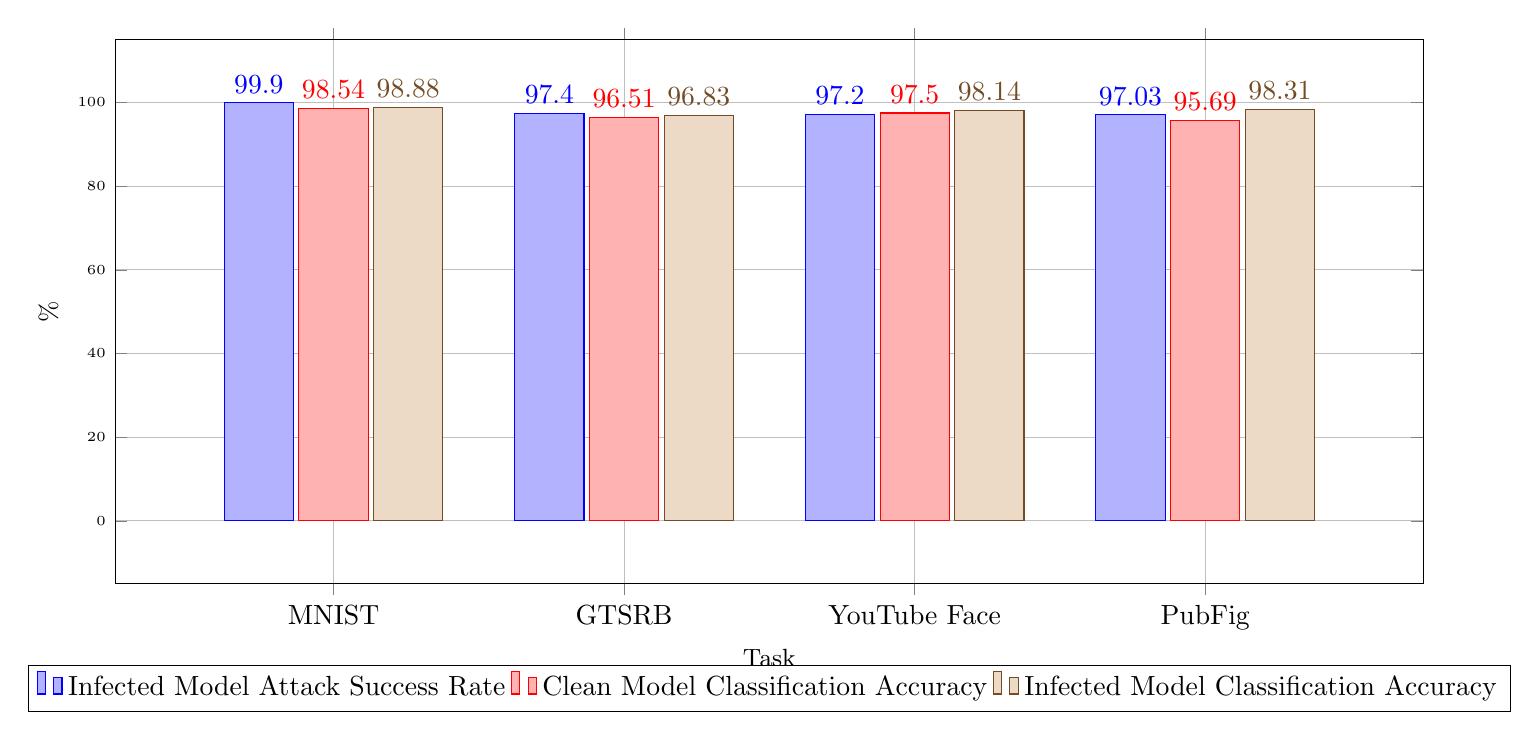
\begin{tikzpicture}
            \begin{axis}[
                ybar=2pt, 
                symbolic x coords={MNIST, GTSRB, YouTube Face, PubFig}, 
                xtick=data, 
                ylabel={\%}, 
                xlabel={Task},
                width=1.5\textwidth, % Adjust width to 60% of text width for proper centering
                height=0.7\textwidth, % Adjust height to maintain aspect ratio
                bar width=25pt, % Slightly larger bars for better visibility
                enlarge x limits=0.25, 
                ymin=0, ymax=100, 
                nodes near coords, 
                nodes near coords align={vertical},
                grid=major,
                every axis label/.append style={font=\small},
                every axis tick label/.append style={font=\small},
                legend style={at={(0.5,-0.15)}, anchor=north, legend columns=-1},
                yticklabel style={font=\tiny},
                enlarge y limits=0.15
            ]

            % Infected Model Attack Success Rate (First Slide)
            
                \addplot coordinates {(MNIST, 99.90) (GTSRB, 97.40) (YouTube Face, 97.20) (PubFig, 97.03)};
                \addlegendentry{Infected Model Attack Success Rate}
            
            
            % Clean Model Classification Accuracy (Second Slide)
            
                \addplot coordinates {(MNIST, 98.54) (GTSRB, 96.51) (YouTube Face, 97.50) (PubFig, 95.69)};
                \addlegendentry{Clean Model Classification Accuracy}
            
            
            % Infected Model Classification Accuracy (Third Slide)
            
                \addplot coordinates {(MNIST, 98.88) (GTSRB, 96.83) (YouTube Face, 98.14) (PubFig, 98.31)};
                \addlegendentry{Infected Model Classification Accuracy}
            
            
            \end{axis}
        \end{tikzpicture}
        }
    \end{figure}
    }
\end{frame}





\begin{frame}{Backdoor Detection Performance}

    \begin{itemize}
        \item<1-> \textbf{\textcolor{red}{Detection success rate}}: \textcolor{blue}{High anomaly index observed} for \textbf{\textcolor{red}{infected models}}.
        \pause
        \item<2-> \textbf{\textcolor{red}{L1 norm of the trigger}}: \textcolor{blue}{Optimized triggers exhibit low L1 norm}, highlighting \textcolor{blue}{sparsity} in their \textcolor{blue}{patterns}.
        \pause
        % \item \textcolor{red}{Reverse-engineered triggers closely match original ones}.
    \end{itemize}

    \begin{figure}[h!]
        \centering
        % First subfigure
        \only<3->{
        \begin{subfigure}{0.45\textwidth}
            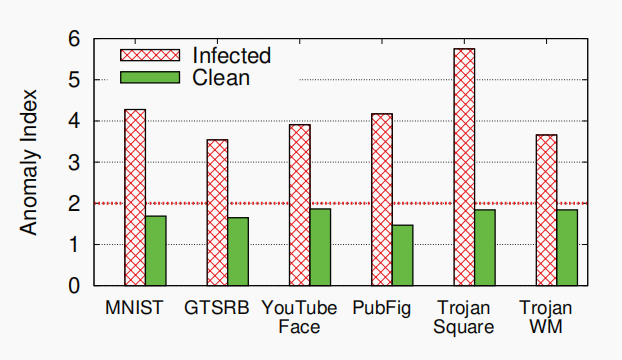
\includegraphics[width=\textwidth]{anomalyIndex.png} % Replace with your first image
            \caption{Anomaly measurement of infected and clean model}
            \label{fig:trigger1}
        \end{subfigure}
        \hfill
        % Second subfigure
        \begin{subfigure}{0.45\textwidth}
            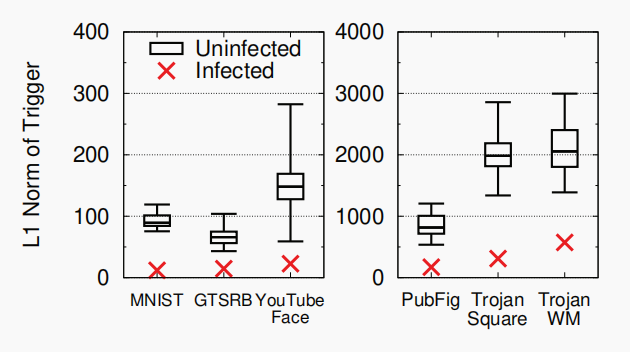
\includegraphics[width=\textwidth]{L1Norm.png} % Replace with your second image
            \caption{L1 norm of triggers for infected and uninfected labels}
            \label{fig:trigger2}
        \end{subfigure}
        \caption{Comparison of trigger visualizations.}
        \label{fig:trigger_visualizations}
        }
    \end{figure}

\end{frame}

\begin{frame}{Identification of Original Triggers}

    \begin{itemize}
        \item<1-> \textbf{\textcolor{red}{End-to-End Effectiveness}} 
        \item<2-> \textbf{\textcolor{blue}{Visual Similarity}} 
        \item<3-> \textbf{\textcolor{red}{Compactness of the Trigger}} 
        \item<4-> \textbf{\textcolor{blue}{Model Behavior}}
    \end{itemize}

     % Figures appear after all points
    \begin{figure}[h!]
        \centering
        % \only<5->{ % Figures will only be visible on the fifth step
            \begin{subfigure}{0.3\textwidth}
                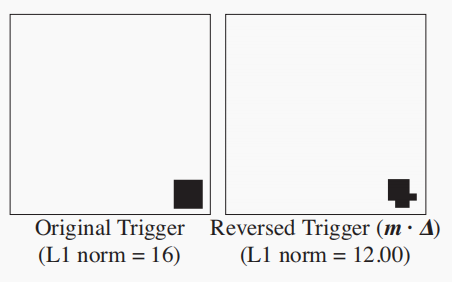
\includegraphics[width=\textwidth]{MNIST.png} % Replace with your first image
                \caption{MNIST}
                \label{fig:revtrigger1}
            \end{subfigure}
            \hfill
            \begin{subfigure}{0.3\textwidth}
                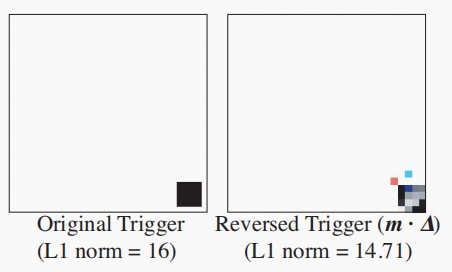
\includegraphics[width=\textwidth]{GTSRB.png} % Replace with your second image
                \caption{GTSRB}
                \label{fig:revtrigger2}
            \end{subfigure}
            \hfill
            \begin{subfigure}{0.3\textwidth}
                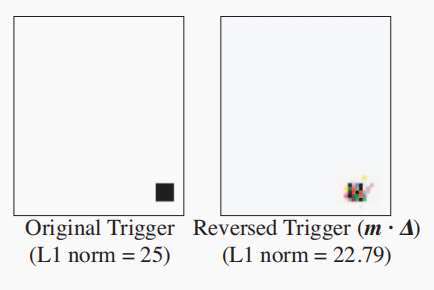
\includegraphics[width=\textwidth]{utubeface.png} % Replace with your third image
                \caption{YouTube Face}
                \label{fig:revtrigger3}
            \end{subfigure}
            \hfill
            \begin{subfigure}{0.3\textwidth}
                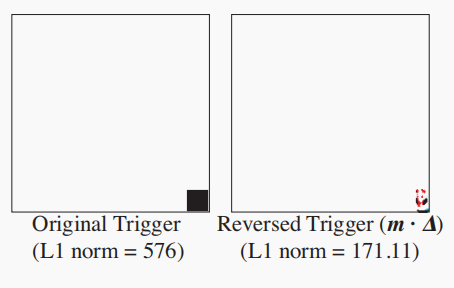
\includegraphics[width=\textwidth]{PubFig.png} % Replace with your fourth image
                \caption{PubFig}
                \label{fig:revtrigger4}
            \end{subfigure}
            \hfill
            \begin{subfigure}{0.3\textwidth}
                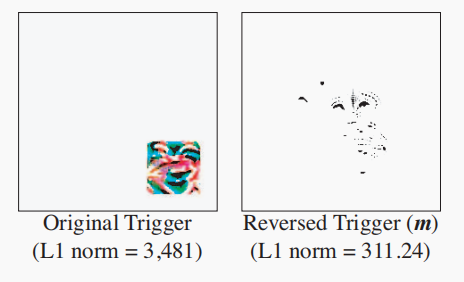
\includegraphics[width=\textwidth]{TrojanSquare.png} % Replace with your fifth image
                \caption{Trojan Square}
                \label{fig:revtrigger5}
            \end{subfigure}
            \hfill
            \begin{subfigure}{0.3\textwidth}
                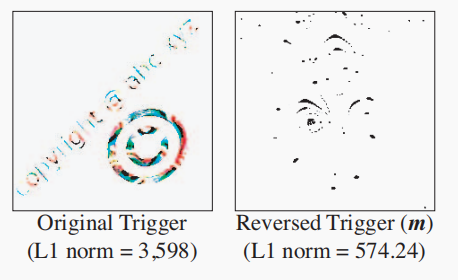
\includegraphics[width=\textwidth]{TrojanWatermark.png} % Replace with your sixth image
                \caption{Trojan Watermark}
                \label{fig:revtrigger6}
            \end{subfigure}
        
        \caption{ Comparison between original trigger and reverse engineered trigger}
        \label{fig:trigger_visualizations}
        % }
    \end{figure}

\end{frame}


% Section 6
\section{Mitigation Techniques}
\subsection{A Simple Example}

\begin{frame}{Mitigation Procedure}

    % First TikZ diagram (Top-left)
    \onslide<1->{
        \begin{tikzpicture}[remember picture, overlay]
            \node[anchor=north west] at ([xshift=0.5cm, yshift=-1.2cm]current page.north west) {
                \resizebox{0.4\textwidth}{!}{
                    \begin{tikzpicture}[scale=0.5, every node/.style={transform shape}]
                        % Frame around network
                        \node[draw, thick, rounded corners, inner sep=1cm, minimum width=10cm, minimum height=6cm, label={[font=\Large]north:Backdoor Model (impurity)}] (frame) at (0,0) {};

                        % Style definitions
                        \tikzset{
                            neuron/.style={circle, draw, minimum size=0.8cm, thick, font=\small, text=black, fill=#1},
                            input neuron/.style={neuron=blue!40},
                            hidden neuron/.style={neuron=green!40},
                            output neuron/.style={neuron=red!40},
                            connection/.style={->, thick},
                        }

                        % Input layer
                        \node[input neuron] (I1) at (0.5, -2) {Input 1};
                        \node[input neuron] (I2) at (0.5, -4) {Input 2};

                        % Hidden layer
                        \node[hidden neuron] (H1) at (4, -1) {H1};
                        \node[hidden neuron] (H2) at (4, -3) {H2};
                        \node[hidden neuron] (H3) at (4, -5) {H3};

                        % Output layer
                        \node[output neuron] (O1) at (8, -3) {Output};

                        % Connections: Input -> Hidden
                        \foreach \i in {I1, I2}
                            \foreach \h in {H1, H2, H3}
                                \draw[connection, blue!60!black] (\i) -- (\h);

                        % Connections: Hidden -> Output
                        \foreach \h in {H1, H2, H3}
                            \draw[connection, green!60!black] (\h) -- (O1);
                    \end{tikzpicture}
                    
                }
            };
        \end{tikzpicture}
        }

        % Image placement (below the TikZ diagram)
    % \onslide<1->{
    %     \begin{tikzpicture}[remember picture, overlay]
    %         \node[anchor=north west, yshift=-6.5cm] at ([xshift=0.5cm, yshift=-7.7cm]current page.north west) { 
    %             
\includegraphics[width=0.4\textwidth]{kkcw_6cco_230518.jpg}
    %         };
    %     \end{tikzpicture}
    % }

    % Second TikZ diagram (Top-right)
    \onslide<2->{
        \begin{tikzpicture}[remember picture, overlay]
            \node[anchor=north east] at ([xshift=-0.5cm, yshift=-1.2cm]current page.north east) {
                \resizebox{0.3\textwidth}{!}{
                    \begin{tikzpicture}

                        % Define node styles
                        \tikzset{
                            neuron/.style={circle, draw=red, very thick, minimum size=1cm, inner sep=0, fill=white},
                            connection/.style={thick, red, dashed},
                            diamond frame/.style={draw=red, thick, rounded corners=1cm, minimum width=5cm, minimum height=5cm}
                        }

                        % Diamond-shaped frame
                        \node[diamond frame] (frame) at (0,0) {};

                        % Neurons (placed symmetrically within the diamond)
                        \node[neuron] (A) at (-0.5, -0.4) {};   % Top
                        \node[neuron] (B) at (-0.5, -2.3) {};   % Right
                        \node[neuron] (C) at (-0.5, -4) {};     % Bottom
                        \node[neuron] (D) at (-4, -2) {};       % Left

                        % Connections (dashed lines)
                        \draw[connection] (A) -- (B);
                        \draw[connection] (A) -- (D);
                        \draw[connection] (B) -- (C);
                        \draw[connection] (B) -- (D);
                        \draw[connection] (C) -- (D);

                    \end{tikzpicture}
                }
            };
        \end{tikzpicture}
    }

    % Third TikZ diagram (Bottom-center)
    \onslide<3->{
        \begin{tikzpicture}[remember picture, overlay]
            \node[anchor=south] at ([xshift=0.5cm, yshift=0.5cm]current page.south) {
                \resizebox{0.4\textwidth}{!}{
                    \begin{tikzpicture}[scale=0.5, every node/.style={transform shape}]
                        % Frame around network
                        \node[draw, thick, rounded corners, inner sep=0.8cm, minimum width=8cm, minimum height=6cm, 
                        label={[font=\Large]south:Clean Model (without impurity)}] (frame) at (0,0) {};

                        % Style definitions
                        \tikzset{
                            neuron/.style={circle, draw, thick, font=\footnotesize, minimum size=0.6cm, text=black, fill=#1},
                            input neuron/.style={neuron=blue!40},
                            hidden neuron/.style={neuron=green!40},
                            output neuron/.style={neuron=red!40},
                            connection/.style={->, thick},
                        }

                        % Input layer (adjusted positions)
                        \node[input neuron] (I1) at (-3, 4.5) {Input 1};
                        \node[input neuron] (I2) at (-3, 2.5) {Input 2};

                        % Hidden layer (adjusted positions)
                        \node[hidden neuron] (H1) at (0,5) {H1};
                        \node[hidden neuron] (H2) at (0, 3.5) {H2};
                        \node[hidden neuron] (H3) at (0, 1.8) {H3};

                        % Output layer (adjusted positions)
                        \node[output neuron] (O1) at (3, 4) {Output};

                        % Connections: Input -> Hidden
                        \foreach \i in {I1, I2}
                            \foreach \h in {H1, H2, H3}
                                \draw[connection, blue!60!black] (\i) -- (\h);

                        % Connections: Hidden -> Output
                        \foreach \h in {H1, H2, H3}
                            \draw[connection, green!60!black] (\h) -- (O1);
                    \end{tikzpicture}
                }
            };
        \end{tikzpicture}
    }

    % Connecting arrows
    \begin{tikzpicture}[remember picture, overlay]
        \onslide<2->{
            \draw[very thick, red!70!black, ->, decorate, decoration={snake, amplitude=0.5mm, segment length=2mm}, 
                  shorten >=2pt, shorten <=2pt]
                ([xshift=5.4cm, yshift=-3cm]current page.north west) -- 
                ([xshift=-4.2cm, yshift=-3cm]current page.north east)
                node[midway, above, sloped, font=\small\bfseries, color=red!80!black] {Trigger Generation}
                node[midway, below, sloped, font=\small\bfseries, color=blue!80!black] {Using Trigger Model};
        }

        \only<3->{
            \draw[very thick, red!70!black, ->, decorate, decoration={snake, amplitude=0.5mm, segment length=2mm}, 
                  shorten >=2pt, shorten <=2pt] 
                ([xshift=-2cm, yshift=-5cm]current page.north east) 
                to[bend left=45] 
                ([xshift=3cm, yshift=2cm]current page.south)
                node[pos=0.6, xshift=10.5cm, yshift=-0.5cm, font=\small\bfseries, color=red!80!black, rotate=-90] {Unlearning Model};
        }
    \end{tikzpicture}

\end{frame}


\subsection{Filtering Adversarial Inputs Based on Neuron Activation Profiles}
\begin{frame}{Filtering Adversarial Inputs}
    \begin{center}
        \textbf{\large Filtering Adversarial Inputs Based on Neuron Activation Profiles}
    \end{center}

    \resizebox{\textwidth}{!}{ % Resize to fit the slide width
        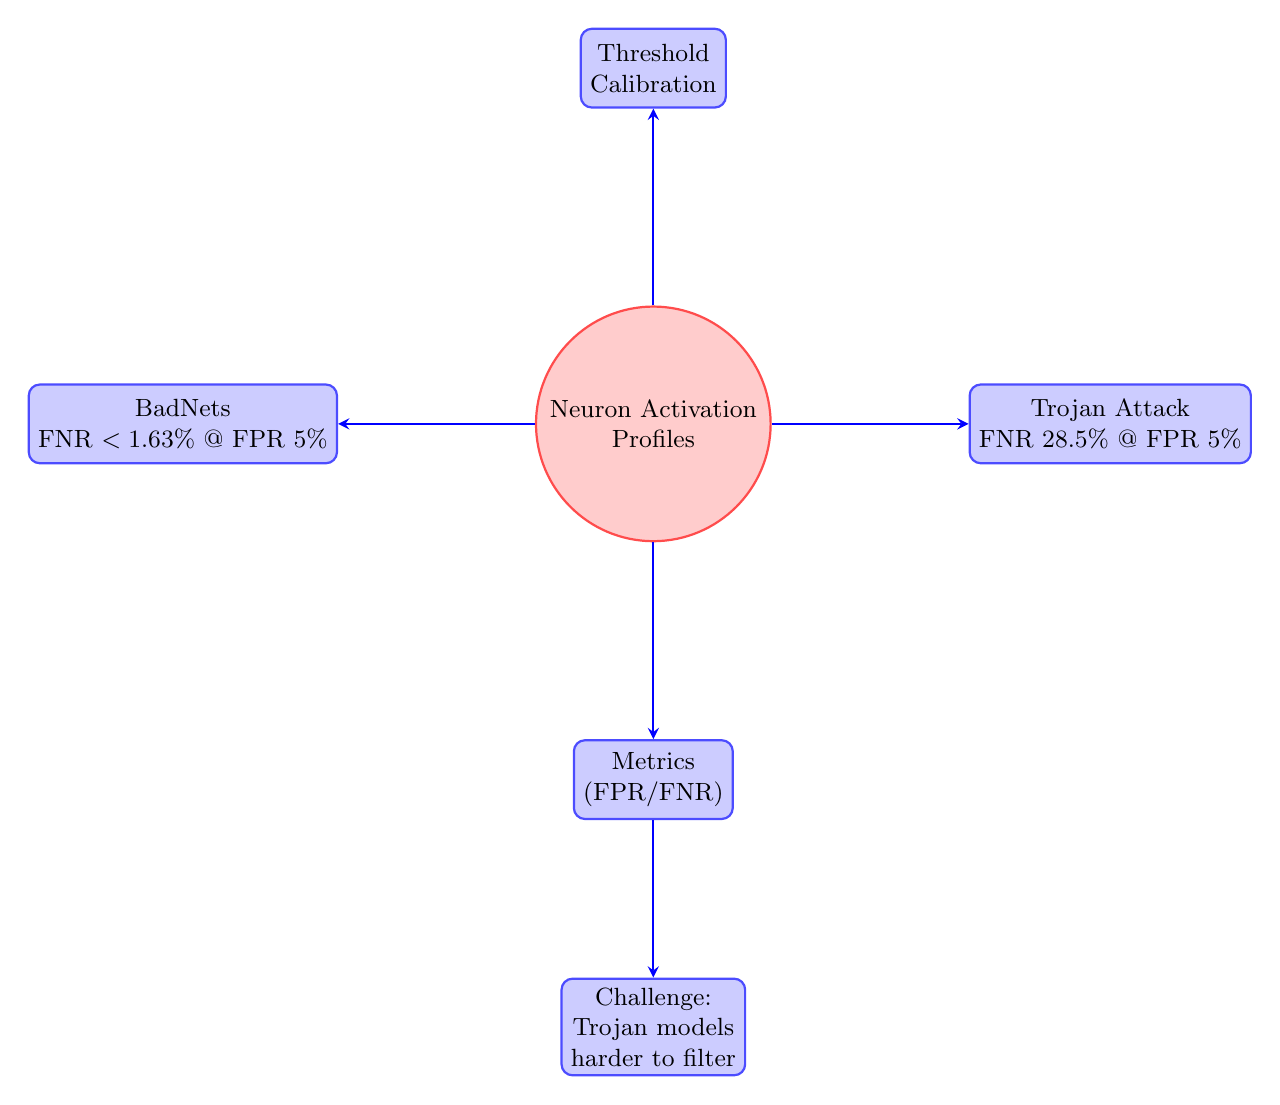
\begin{tikzpicture}[
            node distance=2.5cm,
            every node/.style={font=\small, align=center},
            core/.style={circle, draw=red!70, fill=red!20, thick, minimum size=2cm},
            component/.style={rectangle, draw=blue!70, fill=blue!20, thick, minimum size=1cm, rounded corners},
            arrow/.style={-stealth, thick, blue}
        ]

            % Core element
            \onslide<1->{\node[core] (core) {Neuron Activation \\ Profiles};}

            % Components
            \onslide<2->{\node[component, above=of core] (threshold) {Threshold \\ Calibration};}
            \onslide<3->{\node[component, below=of core] (metrics) {Metrics \\ (FPR/FNR)};}
            \onslide<4->{\node[component, left=of core] (badnets) {BadNets \\ FNR $< 1.63\%$ @ FPR 5\%};}
            \onslide<5->{\node[component, right=of core] (trojan) {Trojan Attack \\ FNR 28.5\% @ FPR 5\%};}
            \onslide<6->{\node[component, below=2cm of metrics] (challenge) {Challenge: \\ Trojan models \\ harder to filter};}

            % Arrows
            \onslide<2->{\draw[arrow] (core) -- (threshold);}
            \onslide<3->{\draw[arrow] (core) -- (metrics);}
            \onslide<4->{\draw[arrow] (core) -- (badnets);}
            \onslide<5->{\draw[arrow] (core) -- (trojan);}
            \onslide<6->{\draw[arrow] (metrics) -- (challenge);}

        \end{tikzpicture}
    }
\end{frame}




\begin{frame}{ROC Curve: Final Visualization}
    \begin{figure}[h]
        \centering
        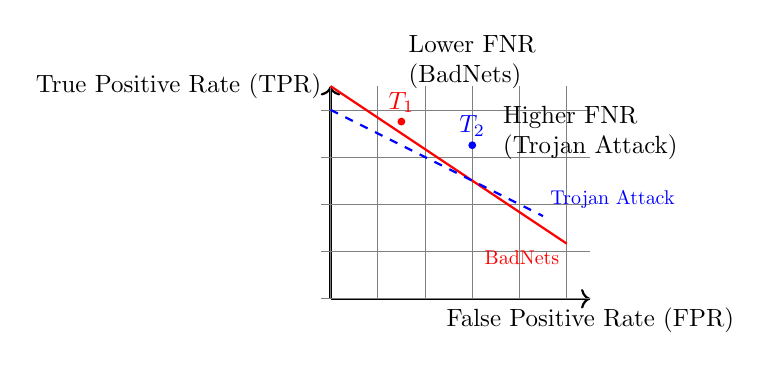
\begin{tikzpicture}[scale=0.6, every node/.style={scale=0.9}]
            % Axes
            \draw[thick,->] (0,0) -- (5.5,0) node[below] {False Positive Rate (FPR)};
            \draw[thick,->] (0,0) -- (0,4.5) node[left] {True Positive Rate (TPR)};
            
            % Grid lines
            \draw[very thin, gray] (-0.2, 0) grid[step=1] (5.5, 4.5);
            
            % BadNets ROC curve (Red)
            \draw[thick,smooth,samples=100,domain=0:5,red] 
            plot(\x,{4.5-\x/1.5}) 
            node[below left, scale=0.8] {\textcolor{red}{BadNets}}; % Red curve with red text

            % Trojan Attack ROC curve (Blue)
            \draw[thick,dashed,smooth,samples=100,domain=0:4.5,blue] 
             plot(\x,{4-\x/2}) 
            node[above right, scale=0.8] {\textcolor{blue}{Trojan Attack}}; % Blue curve with blue text

            % Threshold points
            \filldraw[red] (1.5,3.75) circle (2pt) node[above] {$T_1$};
            \filldraw[blue] (3,3.25) circle (2pt) node[above] {$T_2$};
            
            % Threshold annotations
            \node[align=left] at (5.5,3.5) {Higher FNR \\ (Trojan Attack)};
            \node[align=left] at (3,5) {Lower FNR \\ (BadNets)};
        \end{tikzpicture}
        \caption{Final: ROC Curve Comparison with Thresholds.}
    \end{figure}
\end{frame}
\subsection{Patching DNNs via Neuron Pruning}
\begin{frame}{Patching DNNs via Neuron Pruning (Graphical View)}
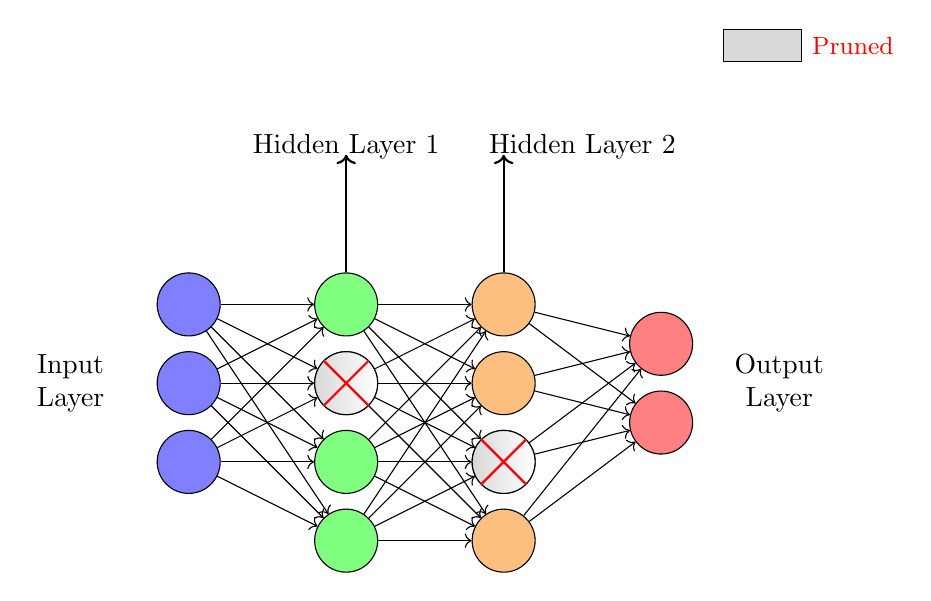
\begin{tikzpicture}[node distance=1cm and 1.5cm, every neuron/.style={circle, draw, minimum size=0.8cm, font=\small}, align=center]

    % Input layer - Blue nodes
    \foreach \i in {1, 2, 3}
        \node[every neuron, fill=blue!50] (I-\i) at (0, -\i) {};

    % Hidden layer 1 - Green nodes
    \foreach \i in {1, 2, 3, 4}
        \node[every neuron, fill=green!50] (H1-\i) at (2, -\i) {};

    % Hidden layer 2 - Orange nodes
    \foreach \i in {1, 2, 3, 4}
        \node[every neuron, fill=orange!50] (H2-\i) at (4, -\i) {};

    % Output layer - Red nodes
    \foreach \i in {1, 2}
        \node[every neuron, fill=red!50] (O-\i) at (6, -\i-0.5) {};

    % Connections from input to hidden layer 1
    \foreach \i in {1, 2, 3}
        \foreach \j in {1, 2, 3, 4}
            \draw[->] (I-\i) -- (H1-\j);

    % Connections from hidden layer 1 to hidden layer 2
    \foreach \i in {1, 2, 3, 4}
        \foreach \j in {1, 2, 3, 4}
            \draw[->] (H1-\i) -- (H2-\j);

    % Connections from hidden layer 2 to output
    \foreach \i in {1, 2, 3, 4}
        \foreach \j in {1, 2}
            \draw[->] (H2-\i) -- (O-\j);

    % Pruned neurons in hidden layer 1 with gray fade
    \node[every neuron, fill=gray!30, shading=axis, left color=gray!30, right color=white] at (2, -2) (H1-pruned) {};
    \draw[thick, red] (H1-pruned.north west) -- (H1-pruned.south east);
    \draw[thick, red] (H1-pruned.north east) -- (H1-pruned.south west);

    % Pruned neurons in hidden layer 2 with gray fade
    \node[every neuron, fill=gray!30, shading=axis, left color=gray!30, right color=white] at (4, -3) (H2-pruned) {};
    \draw[thick, red] (H2-pruned.north west) -- (H2-pruned.south east);
    \draw[thick, red] (H2-pruned.north east) -- (H2-pruned.south west);

    % Adding labels for clarity
    \node[align=center] at (-1.5, -2) {Input\\Layer};
    \node[align=center] at (2, 1) {Hidden Layer 1};
    \node[align=center] at (5, 1) {Hidden Layer 2};
    \node[align=center] at (7.5, -2) {Output\\Layer};

   % Adding rectangular box for "pruned" label for H1-pruned
\node[draw, rectangle, fill=gray!30, minimum height=0.4cm, minimum width=1cm, 
      xshift=5cm, yshift=4cm] at (H1-pruned.north east) (H1-box) {};
\node[align=center, font=\small, text=red, right=0cm of H1-box] {Pruned};
    % Arrows from the 1st neuron of Hidden Layer 1 to its label
    \draw[->, thick] (H1-1) -- (2, 0.9);

    % Arrows from the 1st neuron of Hidden Layer 2 to its label
    \draw[->, thick] (H2-1) -- (4, 0.9);

\end{tikzpicture}
\end{frame}

% Optional fade transition
\transfade[duration=0.5]

\begin{frame}{Patching DNNs via Neuron Pruning (After Removal)}
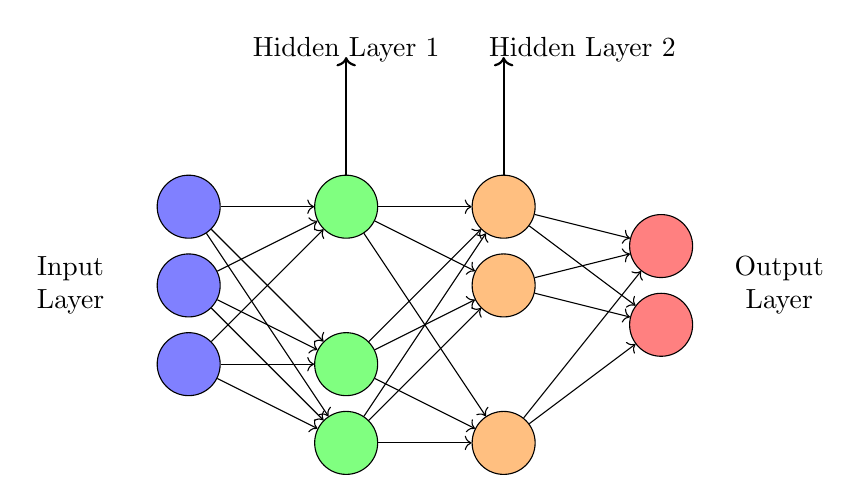
\begin{tikzpicture}[node distance=1cm and 1.5cm, every neuron/.style={circle, draw, minimum size=0.8cm, font=\small}, align=center]

    % Input layer - Blue nodes
    \foreach \i in {1, 2, 3}
        \node[every neuron, fill=blue!50] (I-\i) at (0, -\i) {};

    % Hidden layer 1 - Green nodes (excluding pruned neuron)
    \foreach \i in {1, 3, 4}
        \node[every neuron, fill=green!50] (H1-\i) at (2, -\i) {};

    % Hidden layer 2 - Orange nodes (excluding pruned neuron)
    \foreach \i in {1, 2, 4}
        \node[every neuron, fill=orange!50] (H2-\i) at (4, -\i) {};

    % Output layer - Red nodes
    \foreach \i in {1, 2}
        \node[every neuron, fill=red!50] (O-\i) at (6, -\i-0.5) {};

    % Connections from input to hidden layer 1 (excluding pruned connections)
    \foreach \i in {1, 2, 3}
        \foreach \j in {1, 3, 4}
            \draw[->] (I-\i) -- (H1-\j);

    % Connections from hidden layer 1 to hidden layer 2 (excluding pruned connections)
    \foreach \i in {1, 3, 4}
        \foreach \j in {1, 2, 4}
            \draw[->] (H1-\i) -- (H2-\j);

    % Connections from hidden layer 2 to output
    \foreach \i in {1, 2, 4}
        \foreach \j in {1, 2}
            \draw[->] (H2-\i) -- (O-\j);

    % Adding labels for clarity
    \node[align=center] at (-1.5, -2) {Input\\Layer};
    \node[align=center] at (2, 1) {Hidden Layer 1};
    \node[align=center] at (5, 1) {Hidden Layer 2};
    \node[align=center] at (7.5, -2) {Output\\Layer};

    % % Adding pruned labels
    % \node[align=center, font=\small, text=red] at (2, -2) {Pruned};
    % \node[align=center, font=\small, text=red] at (4, -3) {Pruned};
    % Arrows from the 1st neuron of Hidden Layer 1 to its label
    \draw[->, thick] (H1-1) -- (2, 0.9);

    % Arrows from the 1st neuron of Hidden Layer 2 to its label
    \draw[->, thick] (H2-1) -- (4, 0.9);

\end{tikzpicture}
\end{frame}

\begin{frame}{Patching DNNs via Neuron Pruning}
   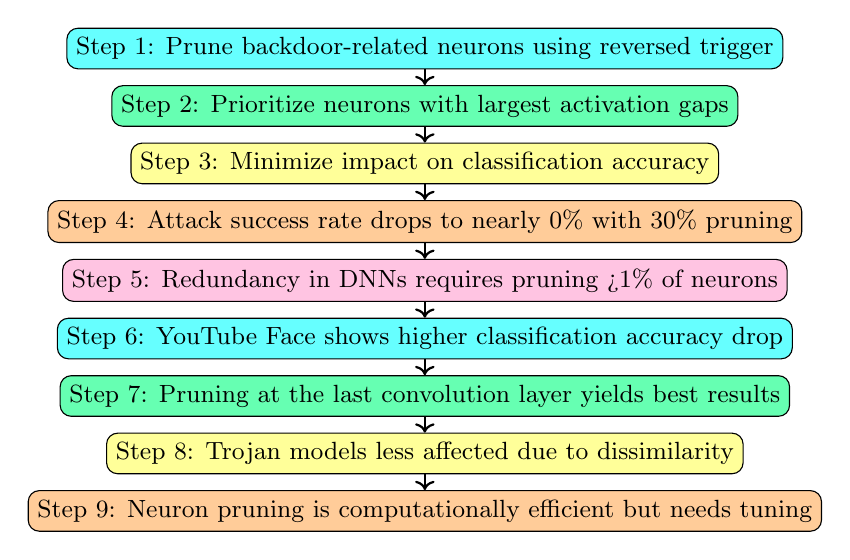
\begin{tikzpicture}[node distance=.2cm, auto, scale=0.8, every node/.style={font=\small}]
        % Define colors
        \definecolor{stepcolor1}{HTML}{66FFFF} 
        \definecolor{stepcolor2}{HTML}{66FFB2} 
        \definecolor{stepcolor3}{HTML}{FFFF99} 
        \definecolor{stepcolor4}{HTML}{FFCC99} 
        \definecolor{stepcolor5}{HTML}{FFC4E2}

        % Flowchart nodes with animations (using \pause)
        \node[draw, fill=stepcolor1, text centered, rounded corners] (step1) {Step 1: Prune backdoor-related neurons using reversed trigger};
        \pause
        \node[draw, fill=stepcolor2, text centered, rounded corners, below=of step1] (step2) {Step 2: Prioritize neurons with largest activation gaps};
        \draw[->, thick] (step1) -- (step2);
        \pause
        \node[draw, fill=stepcolor3, text centered, rounded corners, below=of step2] (step3) {Step 3: Minimize impact on classification accuracy};
        \draw[->, thick] (step2) -- (step3);
        \pause
        \node[draw, fill=stepcolor4, text centered, rounded corners, below=of step3] (step4) {Step 4: Attack success rate drops to nearly 0\% with 30\% pruning};
        \draw[->, thick] (step3) -- (step4);
        \pause
        \node[draw, fill=stepcolor5, text centered, rounded corners, below=of step4] (step5) {Step 5: Redundancy in DNNs requires pruning >1\% of neurons};
        \draw[->, thick] (step4) -- (step5);
        \pause

        
        % Adding more steps to complete the process
        \node[draw, fill=stepcolor1, text centered, rounded corners, below=of step5] (step6) {Step 6: YouTube Face shows higher classification accuracy drop};
        \draw[->, thick] (step5) -- (step6);
        \pause
        \node[draw, fill=stepcolor2, text centered, rounded corners, below=of step6] (step7) {Step 7: Pruning at the last convolution layer yields best results};
        \draw[->, thick] (step6) -- (step7);
        \pause
        \node[draw, fill=stepcolor3, text centered, rounded corners, below=of step7] (step8) {Step 8: Trojan models less affected due to dissimilarity};
        \draw[->, thick] (step7) -- (step8);
        \pause
        \node[draw, fill=stepcolor4, text centered, rounded corners, below=of step8] (step9) {Step 9: Neuron pruning is computationally efficient but needs tuning};
        \draw[->, thick] (step8) -- (step9);
        
    \end{tikzpicture}
\end{frame}

\begin{frame}{Patching DNNs via Neuron Pruning}
    \begin{center}
        \textbf{\large \textcolor{red}{Neuron Pruning} for \textcolor{blue}{Deep Neural Network (DNN) Patching}.}
    \end{center}

    \begin{figure}[h!]
        \centering
        \begin{tabular}[t]{@{}ccc@{}} % [t] aligns the subimages at the top
            % First subimage
            \onslide<1->{
                \begin{subfigure}[t]{0.3\textwidth}
                    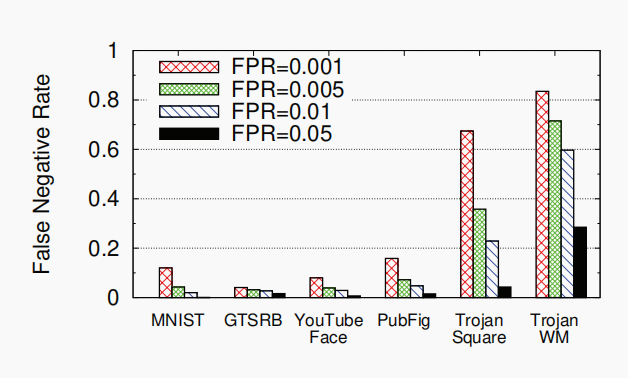
\includegraphics[width=\textwidth]{fnr.png} % Replace with your first image filename
                    \caption{False negative rate of proactive adversarial image detection when achieving different false positive rates.}
                    \label{fig:original_dnn}
                \end{subfigure}
            } &
            % Second subimage
            \onslide<2->{
                \begin{subfigure}[t]{0.3\textwidth}
                    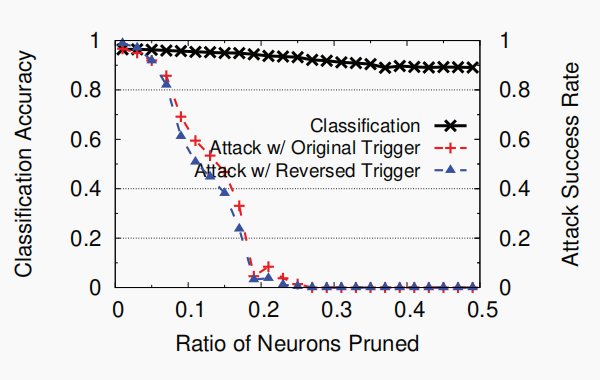
\includegraphics[width=\textwidth]{gtsrb ca and asr.png} % Replace with your second image filename
                    \caption{Classification accuracy and attack success rate when pruning trigger-related neurons in GTSRB (traffic sign recognition w/ 43 labels).}
                    \label{fig:pruning_process}
                \end{subfigure}
            } &
            % Third subimage
            \onslide<3->{
                \begin{subfigure}[t]{0.3\textwidth}
                    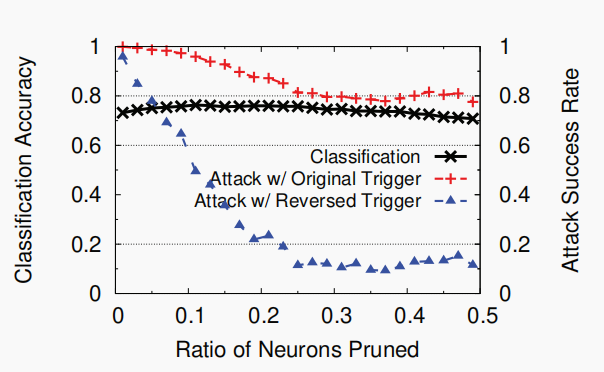
\includegraphics[width=\textwidth]{trojan attack succes rate.png} % Replace with your third image filename
                    \caption{Classification accuracy and attack success rate when pruning trigger-related neurons in Trojan Square (face recognition w/ 2,622 labels).}
                    \label{fig:patched_dnn}
                \end{subfigure}
            }
        \end{tabular}
        \caption{Illustration of Neuron Pruning to Patch DNNs.}
        \label{fig:neuron_pruning}
    \end{figure}
\end{frame}

\begin{frame}{Patching DNNs via Unlearning}
    \begin{figure}[h!]
        \centering
        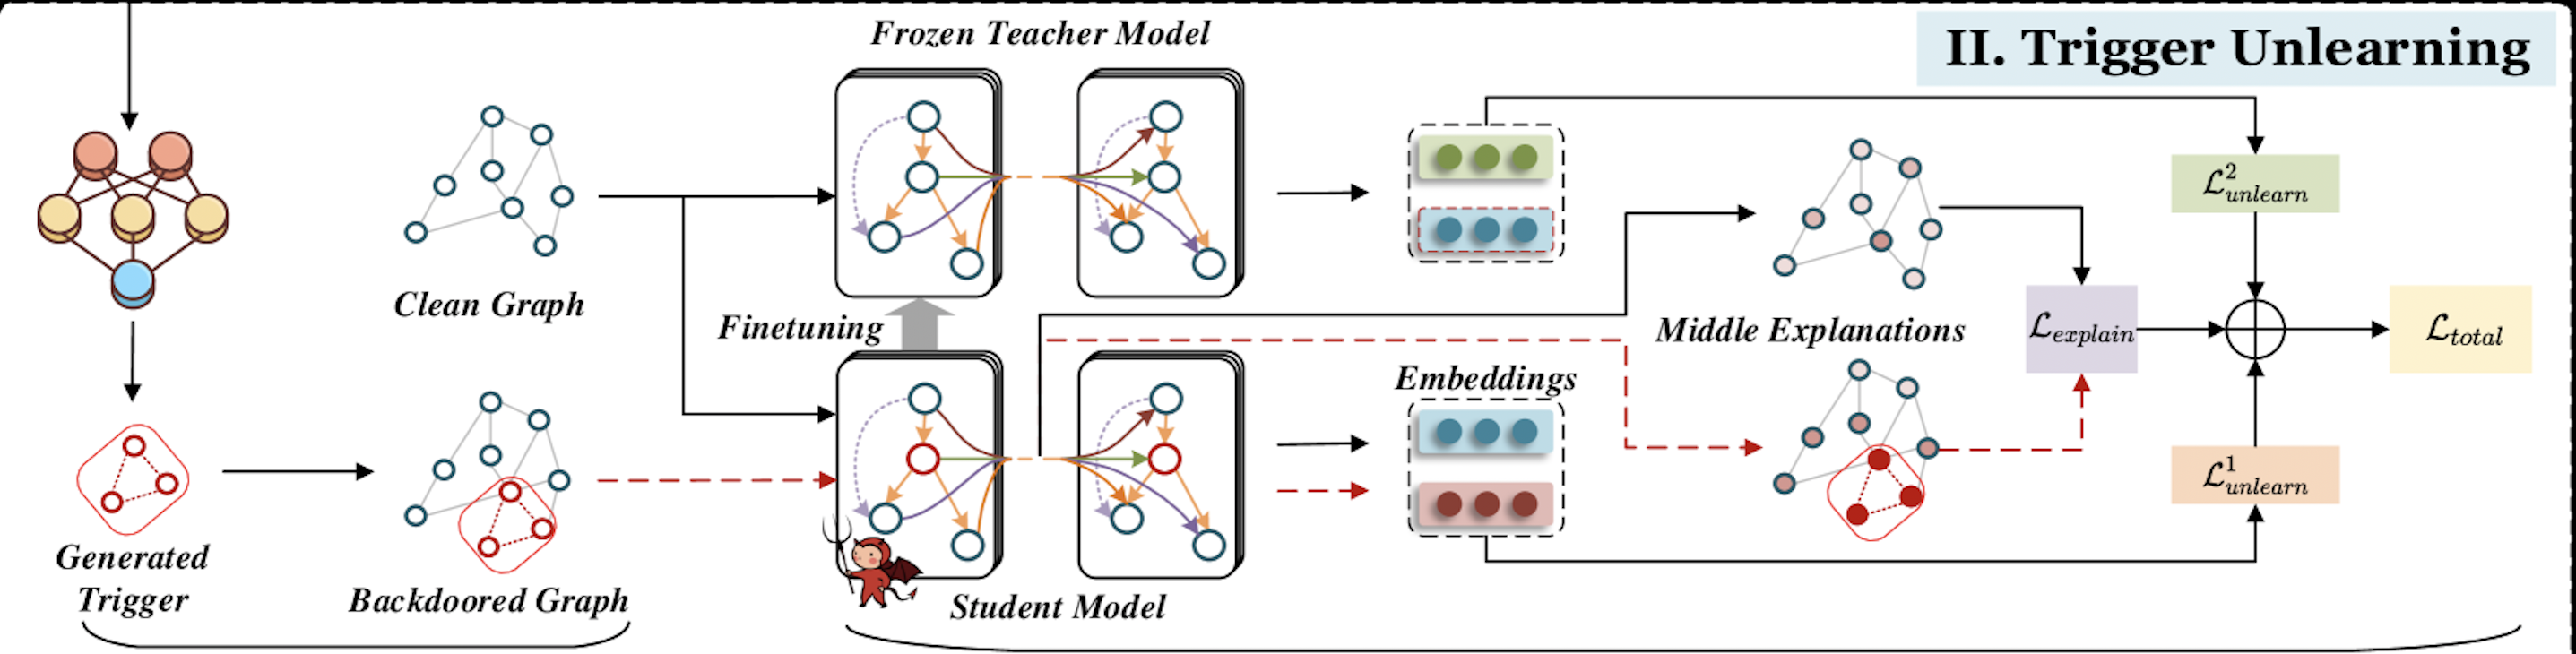
\includegraphics[width=0.9\paperwidth, height=0.9\paperheight, keepaspectratio]{trigger unlearning.png} % Replace "trigger unlearning.png" with your image file
        \caption{Trigger Unlearning graphical visualization}
        \label{fig:trigger_unlearning}
    \end{figure}
\end{frame}




\subsection{Patching DNNs via Unlearning}
\begin{frame}{Patching DNNs via Unlearning}
   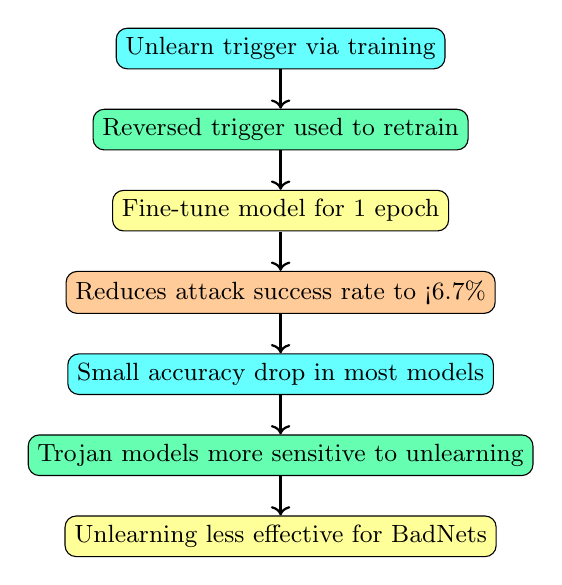
\begin{tikzpicture}[node distance=0.5cm, auto, scale=0.7, every node/.style={font=\small}]
        % Define colors
        \definecolor{stepcolor1}{HTML}{66FFFF} 
        \definecolor{stepcolor2}{HTML}{66FFB2} 
        \definecolor{stepcolor3}{HTML}{FFFF99} 
        \definecolor{stepcolor4}{HTML}{FFCC99} 

        % Keypoint nodes with animations
        \node<1->[draw, fill=stepcolor1, text centered, rounded corners] (step1) {Unlearn trigger via training};
        \node<2->[draw, fill=stepcolor2, text centered, rounded corners, below=of step1] (step2) {Reversed trigger used to retrain};
        \node<3->[draw, fill=stepcolor3, text centered, rounded corners, below=of step2] (step3) {Fine-tune model for 1 epoch};
        \node<4->[draw, fill=stepcolor4, text centered, rounded corners, below=of step3] (step4) {Reduces attack success rate to <6.7\%};
        
        % Connecting the steps with animations
        \draw<2->[->, thick] (step1) -- (step2);
        \draw<3->[->, thick] (step2) -- (step3);
        \draw<4->[->, thick] (step3) -- (step4);

        % Additional keypoints with animations
        \node<5->[draw, fill=stepcolor1, text centered, rounded corners, below=of step4] (step5) {Small accuracy drop in most models};
        \node<6->[draw, fill=stepcolor2, text centered, rounded corners, below=of step5] (step6) {Trojan models more sensitive to unlearning};
        \node<7->[draw, fill=stepcolor3, text centered, rounded corners, below=of step6] (step7) {Unlearning less effective for BadNets};
        
        % Connecting the additional points with animations
        \draw<5->[->, thick] (step4) -- (step5);
        \draw<6->[->, thick] (step5) -- (step6);
        \draw<7->[->, thick] (step6) -- (step7);
   \end{tikzpicture}
\end{frame}
% Slide 1: Classification Accuracy
\begin{frame}{Classification Accuracy After Patching}
    \centering
    \resizebox{1.1\textwidth}{!}{ % Adjust size to fit the slide width
        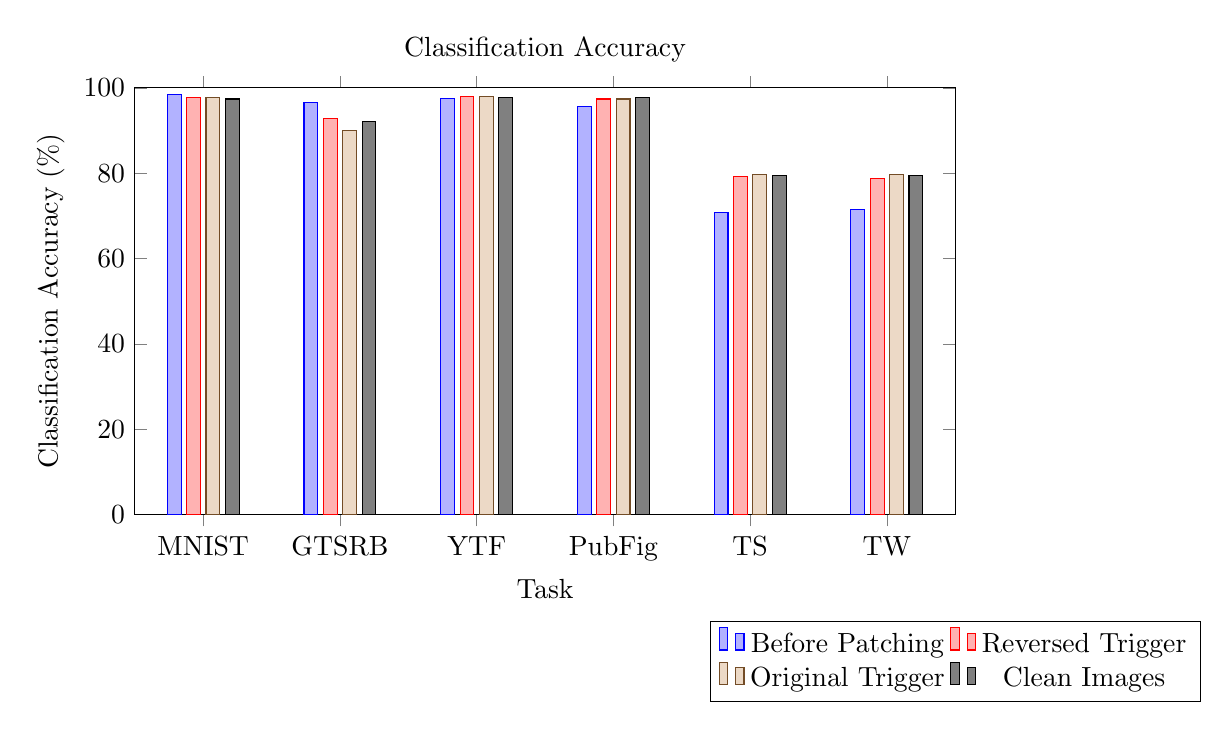
\begin{tikzpicture}
            \begin{axis}[
                ybar,
                bar width=5pt,
                ylabel={Classification Accuracy (\%)},
                symbolic x coords={MNIST, GTSRB, YTF, PubFig, TS, TW},
                xtick=data,
                ymin=0, ymax=100,
                enlarge x limits=0.1,
                width=12cm,
                height=7cm,
                xlabel={Task},
                title={Classification Accuracy},
                legend style={at={(1.0,-0.25)}, anchor=north, legend columns=2},
                legend entries={Before Patching, Reversed Trigger, Original Trigger, Clean Images},
            ]
            \addplot coordinates {(MNIST, 98.54) (GTSRB, 96.51) (YTF, 97.50) (PubFig, 95.69) (TS, 70.80) (TW, 71.40)};
            \addplot coordinates {(MNIST, 97.69) (GTSRB, 92.91) (YTF, 97.90) (PubFig, 97.38) (TS, 79.20) (TW, 78.80)};
            \addplot coordinates {(MNIST, 97.77) (GTSRB, 90.06) (YTF, 97.90) (PubFig, 97.38) (TS, 79.60) (TW, 79.60)};
            \addplot coordinates {(MNIST, 97.38) (GTSRB, 92.02) (YTF, 97.80) (PubFig, 97.69) (TS, 79.50) (TW, 79.50)};
            \end{axis}
        \end{tikzpicture}
    }
\end{frame}

% Optional fade transition
\transfade[duration=0.5]

% Slide 2: Attack Success Rate
\begin{frame}{Attack Success Rate After Patching}
    \centering
    \resizebox{1.1\textwidth}{!}{ % Adjust size to fit the slide width
        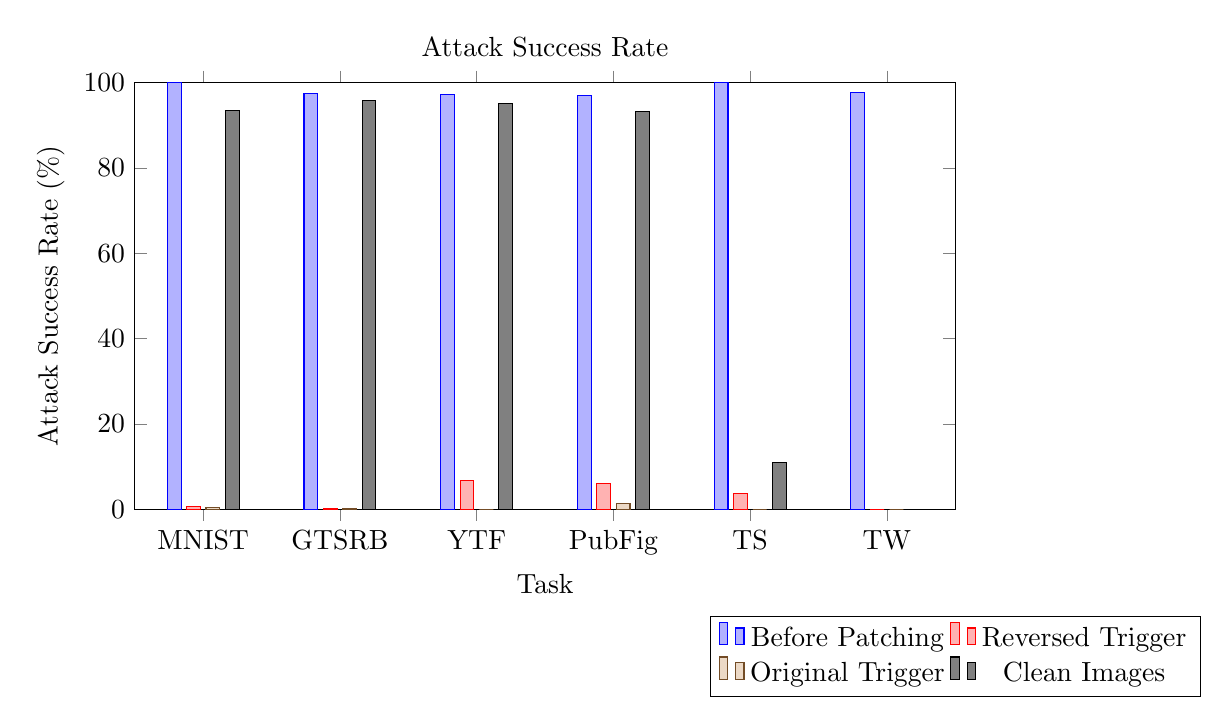
\begin{tikzpicture}
            \begin{axis}[
                ybar,
                bar width=5pt,
                ylabel={Attack Success Rate (\%)},
                symbolic x coords={MNIST, GTSRB, YTF, PubFig, TS, TW},
                xtick=data,
                ymin=0, ymax=100,
                enlarge x limits=0.1,
                width=12cm,
                height=7cm,
                xlabel={Task},
                title={Attack Success Rate},
                legend style={at={(1.0,-0.25)}, anchor=north, legend columns=2},
                legend entries={Before Patching, Reversed Trigger, Original Trigger, Clean Images},
            ]
            \addplot coordinates {(MNIST, 99.90) (GTSRB, 97.40) (YTF, 97.20) (PubFig, 97.03) (TS, 99.90) (TW, 97.60)};
            \addplot coordinates {(MNIST, 0.57) (GTSRB, 0.14) (YTF, 6.70) (PubFig, 6.09) (TS, 3.70) (TW, 0.00)};
            \addplot coordinates {(MNIST, 0.29) (GTSRB, 0.19) (YTF, 0.00) (PubFig, 1.41) (TS, 0.00) (TW, 0.00)};
            \addplot coordinates {(MNIST, 93.37) (GTSRB, 95.69) (YTF, 95.10) (PubFig, 93.30) (TS, 10.91) (TW, 0.00)};
            \end{axis}
        \end{tikzpicture}
    }
\end{frame}

\end{document}
